\documentclass[12pt]{article}
\usepackage{graphicx}
\usepackage{amsmath}
\usepackage{amssymb}
\usepackage{color}
\usepackage{caption}
\usepackage{subcaption}
\usepackage{mdframed}
\usepackage[margin=3cm]{geometry}
\usepackage[superscript,nomove]{cite}
\numberwithin{equation}{section}
\numberwithin{figure}{section}
\usepackage[makeroom]{cancel}
\usepackage{textcomp}
\usepackage{gensymb}
\DeclareMathOperator\arctanh{arctanh}
\usepackage[colorlinks=true]{hyperref}
\usepackage{cleveref}
\crefdefaultlabelformat{[#2#1#3]}
\begin{document}
\renewcommand\citeform[1]{[#1]}
%
\title{MSc Data Science Project: Can a Convolutional Neural Network judge a book by its cover?}
\author{\\Ryan Hill MSci\\\\
Supervisor: Dr Hubie Chen\\\\
Birkbeck, University Of London\\\\
\texttt{rhill06@mail.bbk.ac.uk}}
\date{\today}
\maketitle
\thispagestyle{empty}
\graphicspath{{images/}}
\begin{abstract}
	Coming soon...
\end{abstract}
\begin{figure}[!b]
	\centering
	
\includegraphics[scale=0.4]{bbk_logo.jpg}
\end{figure}

\clearpage
%
{\hypersetup{linkcolor=black}
\tableofcontents}
\thispagestyle{empty}
\clearpage
%
\setcounter{page}{1}
\section{Introduction} 
\label{sec:intro}

Introduce the project, describe the goal and the idea behind why this is important. Explain the structure of this work,

\subsection{Related Works} 
\label{sub:Related Works} 
Discuss the work of Iwana as the main source, reference their methods and results but keep much for later where relevant for comparison with my work.
% subsection Related Works end 
% section CNN Theory and Architectures
\section{Theory} 
\label{sec:Theory} 
\subsection{Components of Convolutional Neural Networks} 
\label{sub:Components_of_Convolutional_Neural_Networks} 
Describe the maths and the theory behind the various components of CNNs to the best of my ability, referring to the source papers for more complex combined units where sensible. 
% subsection Components_of_Convolutional_Neural_Networks end 
\subsection{Transfer Learning} 
\label{sub:Transfer_Learning} 
Describe the theory and maths behind transfer learning to the reader.
% subsection Transfer_Learning end 

\subsection{Activation Maximisation} 
\label{sub:Activation_Maximisation} 
Describe the theory and/or maths of activation maximisation and the methods used within the package we use the regularisations applied. 
% subsection Activation_Maximisation end 
% section Theory end 
\section{Data collection and pre-processing} 
\label{sec:Data_collection_and_pre-processing} 
\subsection{Image Download and Manual Review} 
\label{sub:Image Download and Manual Review} 
The 207, 572 images within the complete book32 dataset covering all original 32 classes were downloaded at full resolution using a slightly altered version of the script provided within the Iwana repository \cite{iwanarepo}. The original csv containing all image URLs was split into files of no more than 20,000 records each to allow to the downloads to be run over multiple sessions do to the slow data transfer rates and the overhead of reading data between Google Drive and Google Colab meaning that even checking before downloading an individual file was not much faster than downloading and writing the file anyway. Each sub-file was then iterated over using the remainder of the original script, downloading each image into a sub-folder of the class for that image i.e. the genre classification.

Once all images were downloaded a sample few were manually checked to verify as best as possible that the data was still correct and the downloads has worked. At this point we attempted to identify if any records used in the bookcover30 train or test datasets were actually boxsets, and as such would likely have an unrepresentative cover image, and example of such an image can be seen in \textcolor{red}{TODO: add image}\cref{fig:TBC}. The terms used in a regex search of the titles were \emph{"boxed set", "boxset", "box set", "anthology", "bundle", "\#-book", "\# book"}. 264 records within the bookcover30 dataset matched at least one of these terms and were extracted into a new folder for manual review. The process was somewhat subjective but as a rule of thumb we rejected any image that was not a single front facing cover, that contained pictures of multiple books and was not an arrangement of covers; single covers that seemed to be specifically designed for a boxset were considered acceptable. In total 94 records needed to be removed due to these rules. To preserve the class balance of the train and test datasets, new records were chosen from the book32 dataset by making like-for-like swaps of the same class; any new covers were also reviewed to ensure they were not boxsets. No verification of the class assignment to images was performed so any errors that existed in the original data would have persisted and we continue to use the single class chosen by the original authors in the case of multi-class books.

We chose to split the training data out into training and validation data using a 90/10 random split per class to ensure class balance in all of the training, validation, and test sets. In total the training set compromised of 46,170 records, the validation set 5130 records, and the test set 5700 records; with 1,539, 171, and 190 records per class respectively. 

% subsection Image Download and Manual Review end 
\subsection{Image Pre-processing Technique} 
\label{sub:Image_Pre-processing_Technique} 

We next used 3 different image preparation methods on the datasets to attempt to identify the method that would lead to the best accuracy within our models. At this stage all methods output an image 299x299 pixels as this was the largest size we would need for any future models. By reducing the image size twice, first now and then again when using a specific model, we were potentially losing some information that would lead to a less accurate model; however we chose to do this to speed up training and testing by having to load much smaller data in compared to the original full sized images. Before pre-processing was done we collected the initial shape and average RGB values of each image for further analysis later.

The first pre-processing method (\emph{NoPrep}) was to simply rescale the image directly down to a 299x299 shape using inter-cubic interpolation \textcolor{red}{TODO: explain this mathematically}. This was chosen at the time as a common all-purpose interpolation method, however after later research this method is often chosen to enlarging images, not shrinking them so the potential to use a better interpolation method could be used in future work.

The second method (\emph{Padded}) was to first pad the images with a symmetric pure white border on either the left/right or top/bottom depending on if the image was portrait or landscape (no padding was done if the image was already a perfect square). These images were then downscaled to 299x299 using the same method as above. The final method (\emph{Cropped}) was to crop the image to a perfect square before the same downscaling method was used. 

Once the images had been processed we used a MobileNetV2 model on each processed training and validation dataset for 30 epochs with an early stopping patience of 15 (i.e. if no improvement was seen in validation accuracy over 15 epochs then we did not continue) and the best model for validation accuracy was kept. The model was trained using the default TensorFlow 2 settings of the adam optimiser with a loss function of sparse categorical cross entropy. More details of the set up are detailed in \cref{sec:Model_Training} as other than the epoch and early stopping the same configuration was used for the main training process. The test results of this model trained on each of the 3 datasets is presented in \cref{tab:preprocres} and the second method, padding the image with a white border, achieved the best result on the test data of 15.81\% accuracy. 

\begin{table}[]
	\centering
	\begin{tabular}{|l|r|r|}
	\hline
	\textbf{Pre-processing Method} & \multicolumn{1}{l|}{\textbf{Best epoch}} & \multicolumn{1}{l|}{\textbf{Test Accuracy}} \\ \hline
	NoPrep                         & 8                                        & 14.39\%                                     \\ \hline
	Padded                         & 6                                        & 15.81\%                                     \\ \hline
	Cropped                        & 5                                        & 12.88\%                                     \\ \hline
	\end{tabular}
	\caption{Results of short training on MobileNetV2 on different image pre-processing methods}
	\label{tab:preprocres}
\end{table}

It is important to note at this point that just because this method achieved the best result for this model in a short number of epochs is no guarantee that this would be the method that achieves the best results in other models or over longer epochs. We use this as a rough benchmark as given the constraints on computing power available to us we were only able to train each model in \cref{sec:Model_Training} once for a reasonable number of epochs, so a decision had to be made. It is also possible that hyperparameter tuning for each of these datasets may have led to different outcomes, but again due to the constraint on resources we decided it best to use domain accepted defaults and as such we progress with the padded dataset.

% section Image_Pre-processing_Technique end 
% section Data_Collection_and_pre-processing end 
\section{Model Training} 
\label{sec:Model_Training} 
\subsection{Configuration} 
\label{sub:Configuration} 
All model architectures consisted of their respective base CNN structure as detailed in \cref{sec:CNN_Architectures} followed by a global average pooling 2D layer to reduce the dimensionality of our tensor and to ensure a flat 1D vector which is fully connected to a 30 neuron output layer with a softmax activation. All models were also trained using the same setup in terms of hyperparameters, optimisers and loss functions; the loss function was sparse categorical cross entropy (sparse due to the usage of a non one-hot encoded target vector), the optimiser was the Adam optimiser \cite{Kingma2015}. The optimiser was used with default hyperparameters as defined within the TensorFlow implementation, the most important being the learning rate with was left at the initial value of 0.001. The reason for the usage of the default hyperparameters and not using a more advanced custom optimiser, such as WAME \cite{Mosca2017}, was due to the constraints on access time to computing power. As is the training already had to be completed across multiple sessions and doing any tuning would have resulted in too large a time required to produce meaningful results; Adam produces decent results with the defaults and so they were used in this work.

The models themselves, MobileNetV2, Inception-ResnetV2, and ResNeXt50 were chosen to represent a wide spread of model capabilities and complexities as highlighted in Figure 1 of the Benchmark Analysis of CNNs completed by Bianco et al\cite{Bianco2018}. MobileNetV2 was chosen as it is a lightweight model designed to be capable of running on mobile devices and was meant to be a low complexity comparison in line with AlexNet (due to no pre-trained version of AlexNet being available within TensorFlow), Inception-ResnetV2 for its high accuracy in other use cases, and ResNeXt50 as a smaller version of one of the newer CNN architectures. These models, combined with the original work done by Iwana et al, span a range of complexity and training speed allowing for a good comparison between performance.

The models were training once using the training data as described in \cref{sub:Image Download and Manual Review} and validated against the validation data split out at the same point. No cross-validation was done due to resource limitations.
% subsection Configuration end 
\subsection{Training Performance} 
\label{sub:Training_Performance} 
The models were each trained with a maximum of 200 epochs and early stopping with a patience of 20 due to the time constraints; in the end all 3 models resulted in early stopping by epoch 104 at most. 

The performance of the models throughout training can be seen in \cref{fig:train_perf} where whilst training accuracy continues to increase over time, the validation accuracy doesn't see as much consistent movement which suggests the model is starting to overfit to the training data as opposed to improving the identification of intrinsic underlying features within the images themselves. Iwana does not report their training accuracy so we are not able to compare the performance of our training with theirs.

\begin{figure}
	\centering
	\captionsetup{justification=centering}
	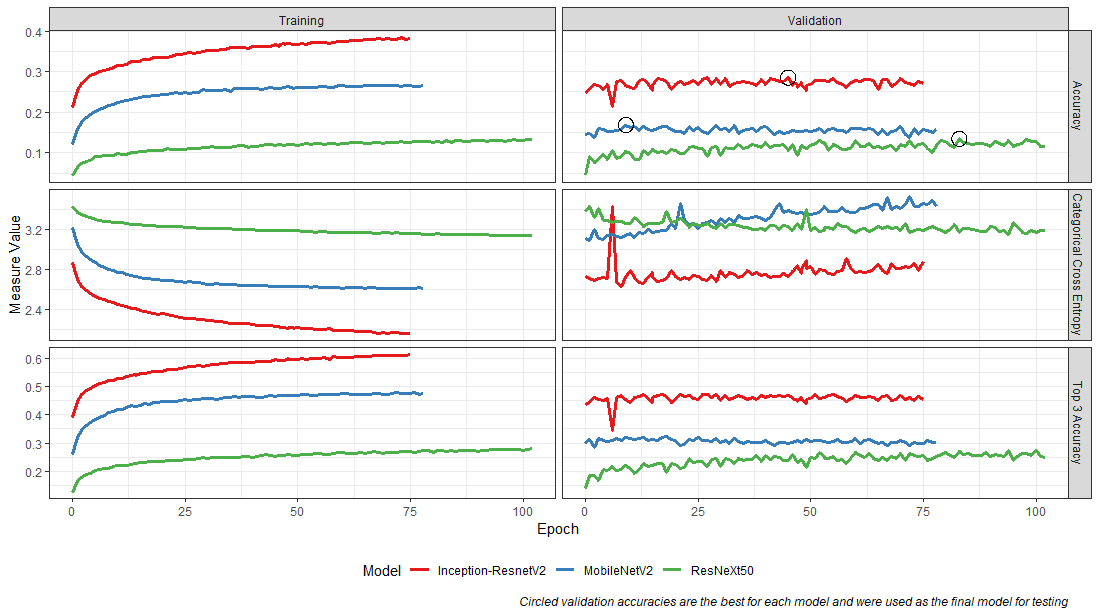
\includegraphics[scale=0.5]{training_results.png}
	\caption{Performance of models on training and validation data throughout training. Note that models that end short stopped training due to early stopping.}
	\label{fig:train_perf}
\end{figure}

Iwana et al trained their models for 30,000 and 450,000 epochs for LeNet and AlexNet respectively, substantially more than we trained our models for, so it is likely that the results they achieved are better than they would have been if they had trained for only a few hundred epochs. It is possible, but not certain, that by training our models for a factor of 10 or 100 more epochs, and removing the early stopping criteria, that we could have achieved even better validation performance.
% subsection Training_Performance end 

% section Model_Training end 

\section{Evaluation} 
\label{sec:Evaluation_and_Further_Exploration} 
\subsection{Results} 
\label{sub:Results} 
Present and discuss the basic results for each model, including a comparison with Iwana with the caveat of a slightly different dataset and different pre-processing. 

% section Results end 
\subsection{Further Analysis} 
\label{sub:Further_Analysis} 
Consider further, in depth, analysis on the best performing model, including some of the insight provided by Iwana.

Idea: compare class average colour by predicted and actual and compare to accuracy?
% section Further_Analysis end 
\subsection{Feature Visualisation} 
\label{sub:Feature_Visualisation} 
Detail the approach taken to try and visualise the ideal input to trigger the most accurate classes in an attempt to understand what feature the model is picking up on. Show output and discuss impact.
% section Feature_Visualisation end  

\subsection{Discussion} 
\label{sub:Discussion} 
Discussion around the reasons we have seen some of these results if not already covered in the previous subsections. 

Future work:
use different interpolation method
% subsection Discussion end 
% section Evaluation_and_Further_Exploration end 

\section{Conclusion} 
\label{sec:Conclusion} 
Discuss the project as a whole, the impact of the results when compared to the literature, and what future work there could be off the back of this.
% section Conclusion end 



%\nocite{*}
\bibliographystyle{ieeetran}
\bibliography{BBK_MSc_Project} 

\appendix

\section{CNN Architectures} 
\label{sec:CNN_Architectures} 
Detail the exact configurations of these architectures
\subsection{MobileNetV2} 
\label{sub:MobileNetV2} 
 
% subsection MobileNetV2 end  
\subsection{Inception-ResnetV2} 
\label{sub:Inception-ResnetV2} 
 
% subsection Inception-ResnetV2 end 
\subsection{ResNeXt50} 
\label{sub:ResNeXt50} 
 
% subsection ResNeXt50 end 
% section CNN_Architectures end 

\section{Technology} 
\label{sec:Technology} 
List of software and packages/libraries including their versions.
% section Technology end 
\end{document}